%-------------------------------------------------------------------------
%
% Latex-Beamer theme for non-commercial/private use
%
% This theme is modified from the theme for
% the University of Twente, by Jasper Goseling.
%
% Author: Xian Qiu
% Date: Oct 4, 2013
% Version: 1.1beta
%
% ------------------------------------------------------------------------

\newcommand{\set}[1]{\left\{#1\right\}}
\newcommand{\norm}[1]{\left\Vert#1\right\Vert}
\newcommand{\abs}[1]{\left\vert#1\right\vert}

\documentclass{beamer}
% Class options include: notes, notesonly, handout, trans,
%                        hidesubsections, shadesubsections,
%                        inrow, blue, red, grey, brown

\usetheme{xq}
\usepackage{tikz}
\usetikzlibrary{arrows,decorations.pathmorphing,backgrounds,positioning,fit,petri}

\title{Fractional Programming in Cooperative Games}
%subtitle is not allowed
\event{Introduction to my PhD work}
\author[Qiu]{Xian Qiu}
\coauthors{Prof. dr. M.J. Uetz\\
           Dr. W. Kern}
% e.g. ``joint work with"
\coauthorstext{Supervised by}
\institute[EWI-DMMP]{Discrete Mathematics and Mathematical Programming Group\\University of Twente}
\footlineauthor{X.Qiu}
\footlineinstitute{University of Twente}
\date[28-08-2013]{Aug 28, 2013}
\footlineleftlogo{U}
\footlinerightlogo{\S}

\begin{document}

\maketitle

\begin{frame}{This is a test frame}
  
  \begin{exampleblock}{Example block}
    This is an example.
  \end{exampleblock}
  
  \begin{alertblock}{Alerted block.}
      \alert{some alerted text.}
  \end{alertblock}

  \begin{block}{Normal block}
    This is a block.
  \end{block}
  
\end{frame}

\section{Introduction}

\begin{frame}\frametitle{An allocation problem}
  Two types of players
  \begin{itemize}
    \item A: Each $i\in A$ possesses an item of size $a_i$
    \item B: Each $j\in B$ possesses a truck of capacity $b_j$
  \end{itemize}

  \pause
  Profit: Proportional to the total size of packed items.

  \pause
  Question: How to allocate the total profit?

  \begin{itemize}
    \item<4-> Fairness
    \item<5-> Cooperative games
  \end{itemize}
\end{frame}

\section{Outline}

\begin{frame}\frametitle{Outline}
  \begin{enumerate}
    \item Cooperative games
    \item<2-> The uniform bin packing game
    \item<3-> Integrality gap
    \item<4-> The non-uniform bin packing game
  \end{enumerate}
\end{frame}

\section{Cooperative games}

\begin{frame}\frametitle{Cooperative games}
  \begin{itemize}
    \item A \emph{cooperative game} $\left<N,v\right>$
      \begin{itemize}
        \item $N$: Player set
        \item $v$: Value function: $v:2^N \rightarrow \mathbb{R}$ satisfying $v(\emptyset)=0$.
      \end{itemize}
    \item<2-> A subset $S \subseteq N$ is called a \emph{coalition}.
    \item<3-> \emph{core}: $x \in \mathbb{R} ^N$ satisfying
    \begin{enumerate}[(i)]
    \item $x(N) = v(N)$,
    \item $x(S)\geq v(S), \forall S\subseteq N$, where $x(S)=\sum_{i\in S}{x_i}$.
    \end{enumerate}
    \item<4-> \emph{(multiplicative) $\epsilon$-core}: Replace (ii) by
      \begin{enumerate}[(ii')]
        \item $x(S)\geq (1-\epsilon)v(S)$.
      \end{enumerate}
      $\epsilon$: \emph{taxation rate}.
    \item<5-> A game is called \emph{$\epsilon$-balanced} if $\epsilon$-core $\neq\emptyset$.
\end{itemize}
\end{frame}

\section{The uniform bin packing game}

\begin{frame}\frametitle{The uniform bin packing game}
  Player set $N$:
  \begin{itemize}
    \item<1-> $k$ bins of capacity 1 each
    \item<2-> $n$ items of size $a_i\in (0,1]$ for $i=1,\cdots,n$
  \end{itemize}
  \pause[3]
  $v(S)$: The maximum total size of items of $S$ which can be packed to the bins of $S$.
  \pause[4]
  \\[10pt]
  \underline{Example}
  \\[10pt]
  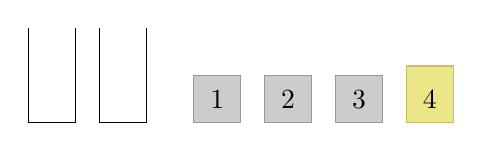
\begin{tikzpicture}[scale = 0.6]

  %%%%%%%%%%%Draw the first bin%%%%%%%%%%%
  \draw (0,0) -- (0,-2);
  \draw (0,-2) -- (1,-2);
  \draw (1,-2) -- (1,0);

  %%%%%%%%%%%Draw the second bin%%%%%%%%%%
  \draw (1.5,0) -- (1.5,-2);
  \draw (1.5,-2) -- (2.5,-2);
  \draw (2.5,-2) -- (2.5,0);

  %%%%%%%%%%%Draw 4 items%%%%%%%%%%%%%%%%%
  \filldraw[fill=gray!40,draw=gray!80] (3.5,-2) rectangle (4.5,-1);
  \draw (4,-1.5) node {1};
  \filldraw[fill=gray!40,draw=gray!80] (5,-2) rectangle (6,-1);
  \draw (5.5,-1.5) node {2};
  \filldraw[fill=gray!40,draw=gray!80] (6.5,-2) rectangle (7.5,-1);
  \draw (7,-1.5) node {3};
  \filldraw[fill=gray!30!yellow!60,draw=yellow!50!gray] (8,-2) rectangle (9,-0.8);
  \draw (8.5,-1.5) node {4};
\end{tikzpicture}
  %%%%%%%%%%%%%%%%Optimum integer packing%%%%%%%%%%%%%%
  \pause
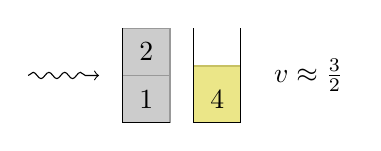
\begin{tikzpicture}[scale = 0.6]
  %right arrow
  \draw [->,decorate, decoration={snake,amplitude=.4mm,segment length=2mm,post length=1mm}]
  (10,-1) -- (11.5,-1);

  \filldraw[fill=gray!40,draw=gray!80] (12,-2) rectangle (13,-1);
  \draw (12.5,-1.5) node {1};
  \filldraw[fill=gray!40,draw=gray!80] (12,-1) rectangle (13,0);
  \draw (12.5,-0.5) node {2};
  \filldraw[fill=gray!30!yellow!60,draw=yellow!50!gray] (13.5,-2) rectangle (14.5,-0.8);
  \draw (14,-1.5) node {4};

  \draw (12,0) -- (12,-2);
  \draw (12,-2) -- (13,-2);
  \draw (13,-2) -- (13,-2);

  \draw (13.5,0) -- (13.5,-2);
  \draw (13.5,-2) -- (14.5,-2);
  \draw (14.5,-2) -- (14.5,0);

  \draw (15,-1) node[right] {$v\approx \frac{3}{2}$};
\end{tikzpicture} 
\end{frame}

\begin{frame}\frametitle{Literature}
  \begin{itemize}
    \item Testing core emptiness and core membership are NP-complete. (Liu 2009)
    \item<2-> $\frac{1}{3}$-core $\neq\emptyset$. (Woeginger 1995)
	  \item<3-> $\frac{1}{7}$-core $\neq\emptyset$ if $a_i>\frac{1}{3}$ (tight bound). (Kuipers 1998)
	  \item<4-> $\epsilon$-core $\neq \emptyset$ if $k\geq O(\epsilon^{-5})$. (Faigle and Kern 1998)
	  \item<5-> $(\frac{1}{3}-\frac{1}{108})$-core $\neq \emptyset$. (Kern and Qiu 2011)
	  \item<6-> $\frac{1}{4}$-core $\neq\emptyset$. (Kern and Qiu 2013)
  \end{itemize}
  \pause
\end{frame}

\section{Integrality gap}
\begin{frame}\frametitle{ILP formulation of $v(N)$}
  \begin{itemize}
     \item Feasible set $F$: Total size $a_F:=\sum_{i\in F}a_i\leq 1$.
     \item<2-> $y_F \in \set{0,1}$.
  \end{itemize}
  \pause[3]
  \begin{align*}
    \text{maximize }   & \sum_{F}a_Fy_F\\
    \text{subject to } & \sum_{F\ni i}y_F\leq 1, \quad i=1,2,\cdots,n,\\
                       & \sum_{F}y_F \leq k,\\
                       & y_F\in\set{0,1}.
  \end{align*}
  \begin{itemize}
    \item<4-> Integrality gap: $\frac{ILP}{LP}$.
  \end{itemize}
\end{frame}

\begin{frame}\frametitle{Non-emptiness of the $\epsilon$-core}
  \begin{itemize}
    \item Integral packing: feasible to ILP\\
          Fractional packing: feasible to LP
    \item<2-> $v$: value of an optimal integral packing\\
              $v'$: value of an optimal fractional packing
  \end{itemize}
\pause[3]
\begin{block}{Lemma 1 (Faigle and Kern [1998])}
$\epsilon$-core($N$)$\neq\emptyset \Leftrightarrow \epsilon\geq 1-\frac{v}{v'}$.
\end{block}
\pause[4]
Trivially, $\frac{1}{2}$-core($N$) $\neq\emptyset$ (for all $N$).
\end{frame}

\section{Frac. packing}

\begin{frame}\frametitle{Fractional packing}
  Fractional packing: $(y'_F)$, satisfying
     \begin{enumerate}[(a)]
        \item $\sum_{F\ni i}{y'_F}\leq 1$, $\forall$ item $i$;
        \item $\sum_{F}y'_F\leq k$.
      \end{enumerate}
      \pause
  \vspace*{10pt}\underline{Example (continue)}
  \\[10pt]
  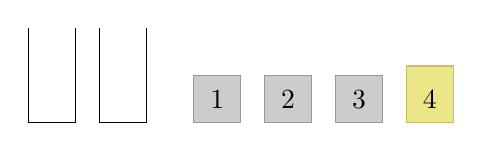
\begin{tikzpicture}[scale = 0.6]

  %%%%%%%%%%%Draw the first bin%%%%%%%%%%%
  \draw (0,0) -- (0,-2);
  \draw (0,-2) -- (1,-2);
  \draw (1,-2) -- (1,0);

  %%%%%%%%%%%Draw the second bin%%%%%%%%%%
  \draw (1.5,0) -- (1.5,-2);
  \draw (1.5,-2) -- (2.5,-2);
  \draw (2.5,-2) -- (2.5,0);

  %%%%%%%%%%%Draw 4 items%%%%%%%%%%%%%%%%%
  \filldraw[fill=gray!40,draw=gray!80] (3.5,-2) rectangle (4.5,-1);
  \draw (4,-1.5) node {1};
  \filldraw[fill=gray!40,draw=gray!80] (5,-2) rectangle (6,-1);
  \draw (5.5,-1.5) node {2};
  \filldraw[fill=gray!40,draw=gray!80] (6.5,-2) rectangle (7.5,-1);
  \draw (7,-1.5) node {3};
  \filldraw[fill=gray!30!yellow!60,draw=yellow!50!gray] (8,-2) rectangle (9,-0.8);
  \draw (8.5,-1.5) node {4};
\end{tikzpicture}
\\[10pt]

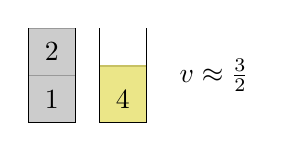
\begin{tikzpicture}[scale = 0.6]
  %%%%%%%%%%%%%%%%Optimum integer packing%%%%%%%%%%%%%%

  \filldraw[fill=gray!40,draw=gray!80] (0,-5) rectangle (1,-4);
  \draw (0.5,-4.5) node {1};
  \filldraw[fill=gray!40,draw=gray!80] (0,-4) rectangle (1,-3);
  \draw (0.5,-3.5) node {2};
  \filldraw[fill=gray!30!yellow!60,draw=yellow!50!gray] (1.5,-5) rectangle (2.5,-3.8);
  \draw (2,-4.5) node {4};

  \draw (0,-3) -- (0,-5);
  \draw (0,-5) -- (1,-5);
  \draw (1,-5) -- (1,-3);

  \draw (1.5,-3) -- (1.5,-5);
  \draw (1.5,-5) -- (2.5,-5);
  \draw (2.5,-5) -- (2.5,-3);

  \node[right] (integral opt) at (3,-4) {$v\approx \frac{3}{2}$};
  
\end{tikzpicture}
%%%%%%%%%%%%%%%%%%%%Optimum fractional packing%%%%%%%%%%%%%
\pause
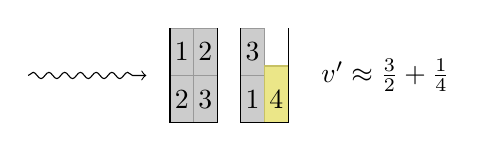
\begin{tikzpicture}[scale =0.6]
  %draw snaked line
  \draw [->,decorate, decoration={snake,amplitude=.4mm,segment length=2mm,post length=1mm}]
  (3,-4) -- (5.5,-4);
  
  \filldraw[fill=gray!40,draw=gray!80] (6,-5) rectangle (6.5,-4);
  \draw (6.25,-4.5) node {2};
  \filldraw[fill=gray!40,draw=gray!80] (6.5,-5) rectangle (7,-4);
  \draw (6.75,-4.5) node {3};
  \filldraw[fill=gray!40,draw=gray!80] (6,-4) rectangle (6.5,-3);
  \draw (6.25,-3.5) node {1};
  \filldraw[fill=gray!40,draw=gray!80] (6.5,-4) rectangle (7,-3);
  \draw (6.75,-3.5) node {2};

  \draw (6,-3) -- (6,-5);
  \draw (6,-5) -- (7,-5);
  \draw (7,-5) -- (7,-3);

  \filldraw[fill=gray!40,draw=gray!80] (7.5,-5) rectangle (8,-4);
  \draw (7.75,-4.5) node {1};
  \filldraw[fill=gray!40,draw=gray!80] (7.5,-4) rectangle (8,-3);
  \draw (7.75,-3.5) node {3};
  \filldraw[fill=gray!30!yellow!60,draw=yellow!50!gray] (8,-5) rectangle (8.5,-3.8);
  \draw (8.25,-4.5) node {4};

  \draw (7.5,-3) -- (7.5,-5);
  \draw (7.5,-5) -- (8.5,-5);
  \draw (8.5,-5) -- (8.5,-3);

  \draw (9,-4) node [right] {$v'\approx \frac{3}{2}+\frac{1}{4}$};

\end{tikzpicture} 
  \\[10pt]
  \pause[4]
  \hspace*{197pt}$1-\frac{v}{v'} \approx \frac{1}{7}$
\end{frame}

\section{The non-uniform bin packing game}
\begin{frame}\frametitle{The non-uniform bin packing game}
  \begin{itemize}
    \item Non-uniform: $1=b_1\geq \cdots\geq b_k$.
    \item<2-> Feasible set $F_j$: $a_{F_j}\leq b_j$.
    \item<3-> $\mathcal{F}_j$: collection of feasible set for bin $j$.
    \item<4-> $\mathcal{F}:=\mathcal{F}_1\supseteq \cdots\supseteq\mathcal{F}_k$ ($\supseteq\mathcal{F}_{k+1} :=\emptyset$).
    \item<5-> $y_F\in\set{0,1}$, $F\in \mathcal{F}$: Pack $F$ or not.
  \end{itemize}
  \pause[6]
  \begin{align*}
    \text{maximize }   & \sum_{F\in\mathcal{F}}a_Fy_F\\
    \text{subject to } & \sum_{F\ni i,F\in\mathcal{F}}y_F\leq 1, \quad i=1,2,\cdots,n,\\
                       & \sum_{F\in \mathcal{F}\backslash \mathcal{F}_{j+1}}y_F \leq j, \quad j = 1,\cdots,k,\\
                       & y_F\in\set{0,1}, \quad \text{for all } F\in\mathcal{F}.
  \end{align*}
\end{frame}

\begin{frame}\frametitle{Literature}
  \begin{itemize}
    \item Results are poor!
    \item<2-> $1/2$-core $\neq\emptyset$ if any item fits any bin. (Faigle and Kern 1995)
    \item<3-> Kern and Qiu (2012) proved the following results:
              \begin{enumerate}
                \item $1/2$-core $\neq\emptyset$.
                \item $5/12$-core $\neq\emptyset$ if $a_i>1/3$.
                \item $\epsilon$-core $\neq\emptyset$ if $k\geq O(\epsilon\bar{b})^{-5}$, where $\bar{b}$ is the average bin capacity.
              \end{enumerate}
  \end{itemize}
\end{frame}


\section{Open questions}
\begin{frame}\frametitle{Open questions}
  \begin{itemize}
    \item Uniform case:\\
      \begin{enumerate}
        \item <2-> $\epsilon_{\min}\in[1/7,1/4]$. Interesting to close the gap.
        \item <3-> $v'-v \leq 1/4$ if $a_i>1/3$. (Faigle and Kern 1998)\\
                   $v'-v \leq C$ in general? (Woeginger)
      \end{enumerate}
    \item<4-> Non-uniform case:\\
      \begin{enumerate}
        \item <4-> Improve the $1/2$ bound.
        \item <5-> Improve the $5/12$ bound for $a_i>1/3$.
      \end{enumerate}
  \end{itemize}
\end{frame}
\end{document}
